\chapter{General discussion}
\label{chapter:discussion}
\chaptermark{General discussion}


% Part~\ref{part:introduction}
% Part~\ref{part:mecfs}
% Chapter~\ref{chapter:statical-challenges-2021}
% Chapter~\ref{chapter:misdiagnosis-serology-2022}
% Chapter~\ref{chapter:impact-misdignosis-2023}
% Chapter~\ref{chapter:2022-revisiting-igg}
% Chapter~\ref{chapter:2023-sym-and-herpesvirus}
% Chapter~\ref{chapter:2024-sym-domains}
% Chapter~\ref{chapter:2021-ace-ace2}
% Part~\ref{part:covid}
% Chapter~\ref{chapter:2022-covid19-01}
% Chapter~\ref{chapter:2023-covid19-02}
% Part~\ref{part:discussion}

% \section{Thesis overview}
% \section{Implications of the results}
% \section{Limitations}
% \section{Further extensions}
% \section{Conclusion}

% general paragraph relating each Part
% \note{General paragraph}
In this thesis, I have presented studies exploring different aspects of myalgic encephalomyelitis/chronic fatigue syndrome (\cfs) as a heterogeneous disease.
% Patient diagnosis agreement of four different case definitions was compared, and case-control study scenarios were simulated to evaluate the implications of misdiagnosis in terms of reproducibility of research findings (Chapter~\ref{chapter:statical-challenges-2021}, Chapter~\ref{chapter:misdiagnosis-serology-2022}, and Chapter~\ref{chapter:impact-misdignosis-2023}).
I compared patient diagnosis agreement between four different case definitions and simulated case-control study scenarios under the assumption of misdiagnosis of patients to evaluate the implications in reproducibility of research findings (Chapter~\ref{chapter:statical-challenges-2021}, Chapter~\ref{chapter:misdiagnosis-serology-2022}, and Chapter~\ref{chapter:impact-misdignosis-2023}).
To study possible links between the immune origin of \cfs, patients were stratified into more homogeneous subgroups related to specific symptom profiles and infection triggers.
They were then compared against healthy controls and multiple sclerosis (MS) patients using data from previously published IgG antibody responses towards antigens of six different herpesviruses and reported symptom assessments
(Chapter~\ref{chapter:2022-revisiting-igg}, Chapter~\ref{chapter:2023-sym-and-herpesvirus}, and Chapter~\ref{chapter:2024-sym-domains}).
This thesis was produced during the \covid pandemic.
As such, I extended the research on \cfs to study the increased risk of \sars infections in \cfs patients (Chapter~\ref{chapter:2021-ace-ace2}) and conducted population studies on the risk of \sars Omicron BA.5 infection in the context of the Portuguese population, a cases study of a highly vaccinated community (Chapter~\ref{chapter:2022-covid19-01} and Chapter~\ref{chapter:2023-covid19-02}).

%%%%%%%%%%%%%%%%%%%%%%%%%%%%%%%%%%%%%%%%%%%%%%%%%%%%%%%%%%%%%%%%%%%%%%%%
%%%%%%%%%%%%%%%%%%%%%%%%%%%%%%%%%%%%%%%%%%%%%%%%%%%%%%%%%%%%%%%%%%%%%%%%
%%%%%%%%%%%%%%%%%%%%%%%%%%%%%%%%%%%%%%%%%%%%%%%%%%%%%%%%%%%%%%%%%%%%%%%%
\section{Misdiagnosis and stratification of ME/CFS}
% \section{Current challenges in ME/CFS}

% ----------------------------------------------------------------------
% ME/CFS case criteria and agreement
% \note{ME/CFS case criteria and agreement}
The analysis of agreement among four of the most commonly used \cfs case definitions revealed that 37.1\% had a disagreement in at least one diagnostic criterion (Chapter~\ref{chapter:statical-challenges-2021}).
This shows how different criteria have distinct focuses for the diagnosis of patients, with varying degrees of inclusiveness \citep{lim2020ReviewCase}.
This uncertainty surrounding diagnosis leads to (relative) misdiagnosis of patients, with an impact on research reproducibility \citep{nacul2019HowHave}.
Considering that currently there is no criterion considered to be a gold standard in either research or clinical practice, a proposed alternative to mitigate possible inconsistencies could be using more than one criterion together.
In fact, when using at least two case definitions, the number of diagnosed individuals greatly improved.
% We have highlighted the lack of agreement among four of the most commonly used ME/CFS case definitions (Chapter~\ref{chapter:statical-challenges-2021}).
% Overall, the definitions overlap sufficiently to diagnose the majority of individuals (62.9\%).
% Nevertheless, the remaining 37.1\% suspected patients receive inconsistent diagnoses, evidencing the difficulty of performing a symptom-based diagnosis---even if combining different case definitions at the same time.
% This uncertainty on the sheer diagnosis leads to (relative) misdiagnosis of patients with an impact on research consistency and reproducibility \citep{nacul2019HowHave}.

% ----------------------------------------------------------------------
% ME/CFS misdiagnosis and stratification
% \note{ME/CFS misdiagnosis and stratification}
% ME/CFS-diagnosed patients exhibit a wide diversity of symptoms and severity degrees \citep{malato2021Statisticalchallenges, domingues2023AssociationAnalysis}, suggesting a heterogeneous aetiology with multiple onset mechanisms proposed as pathogenesis for the disease (see Section~\ref{subsec:pathogenesis}).
% % Additionally, some of the studied mechanisms also share similarities to other diseases, such as MS (see Chapter~\ref{chapter:introduction}).
% This suggests that individuals can reach a diagnosable ME/CFS phenotype through distinct pathways and co-morbidities.
In Chapter~\ref{chapter:statical-challenges-2021}, Chapter~\ref{chapter:misdiagnosis-serology-2022}, and Chapter~\ref{chapter:impact-misdignosis-2023}, I studied how the inclusion of false positive individuals in \cfs cohorts and misclassification negatively impact the consistency of research, particularly in case-control studies.
The findings of these studies highlight \cfs as an example of a challenging illness in terms of research success and reproducibility of results.

% ----------------------------------------------------------------------
% first challenge:
% \note{1st challenge}
The first challenge is that \cfs patient cohorts can be composed of other subgroups, defined as misdiagnosis in a strict sense.
This challenge is directly related to the difficulty in objectively characterising the diagnosed population under the idea that \cfs, being an umbrella term, might encompass distinct subtypes of the disease.
In this sense, I identified the subgroup of false positive cases as having similar characteristics on the candidate causal factor of interest as the matched healthy controls, thus more clearly exemplifying the dilution effect on the statistical power to detect a putative disease association when increasing the misdiagnosis rate (Figure~\ref{fig:stratification-alternatives}, path A).
However, this model does not necessarily impose the idea that apparent cases should be viewed as healthy controls (see Section~\ref{sec:2023-misdiagnosis-discussion}).
Instead, this uncertain group can be viewed as other diseases or specific subgroups of \cfs, both characterised by reduced association or even predisposition to a different causal factor (Figure~\ref{fig:stratification-alternatives}, path B) \citep{nacul2019HowHave}.
% However, this misdiagnosed subgroup does not necessarily indicate healthy individuals (see Section~\ref{sec:2023-misdiagnosis-discussion}).
% Alternatively, apparent cases can be true cases of either another disease or a subgroup of ME/CFS individuals, both characterised by a reduced association or even a predisposition to a different causal factor (Figure~\ref{fig:stratification-alternatives}B) \citep{nacul2019HowHave}.
Under this consideration, the presence probability of the causal factor in suspected \cfs cases would be composed by other specific parametric values, and the $2 \times 2$ tables used to test the null hypothesis would be further augmented.
% Additionally, and as discussed in the study, the cohort of controls can also be split into genuine and apparent controls, further reducing the overall power to detect a putative disease association.

\begin{figure}[h]
    \centering
    % 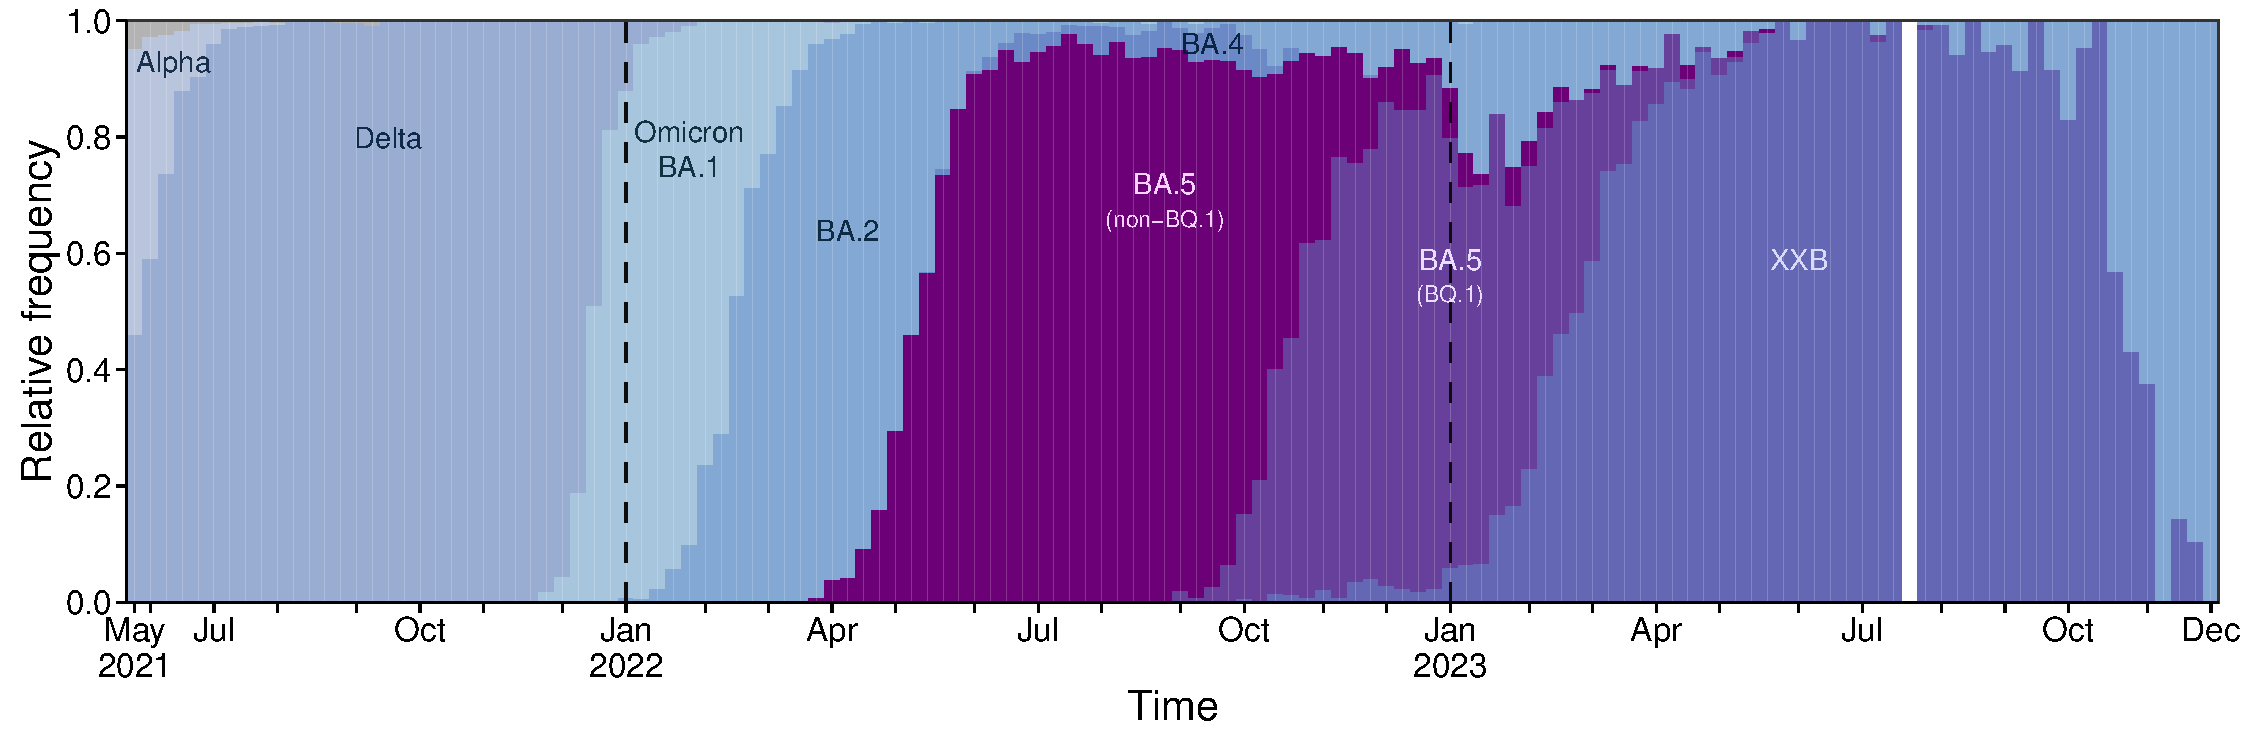
\includegraphics[width=\textwidth]{chapter/introduction/figures/fig1-sarscov2-genetic-diversity-pt.pdf}
    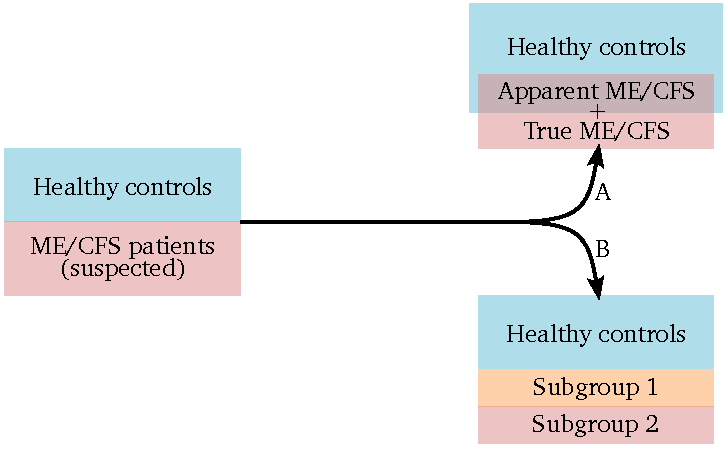
\includegraphics{chapter/discussion/figures/stratification-alternatives.pdf}
    \caption[Alternative misdiagnosis assumptions to include patient stratification]{Alternative misdiagnosis assumptions to include patient stratification. From the initial sample of healthy controls and suspected ME/CFS cases (left box), assumptions can be made as to (A) assess the inclusion of apparent cases (false positives) that are similar to controls regarding the measured causal risk factor; or (B) stratify patients into distinct subgroups with specific distinct parametric values for the risk factor.}
    \label{fig:stratification-alternatives}
\end{figure}
% Figure 2
% Figure~\ref{fig:stratification-alternatives}

% ----------------------------------------------------------------------
% second challenge:
% \note{2nd challenge}
The second challenge stems from the notion that there are likely neither single nor strong associations between a candidate causal factor and ME/CFS \citep{dibble2020GeneticRisk, malato2023ImpactMisdiagnosis}.
Consequently---and aligning with the previous challenge---candidate markers for the disease should be tested on specific subsets of patients.
% that better exemplify the association between cause and effect.
% results on stratification
% \note{Stratification}
% Throughout the thesis, \cfs was stratified
% into more homogeneous subgroups was done based on disease-triggering herpesviruses-related infections and symptoms grouped by mechanistic domains.
Throughout the thesis, \cfs cases were stratified based on disease-triggering herpesviruses-related infections and symptoms grouped by mechanistic domains.
% (Chapter~\ref{chapter:2022-revisiting-igg}, Chapter~\ref{chapter:2023-sym-and-herpesvirus}, and Chapter~\ref{chapter:2024-sym-domains}).
% We analysed data from both a specialised biobank (UKMEB) and published studies.
One approach analysed data on antibody responses against specific peptides from Epstein–Barr virus (EBV) in \cfs patients and healthy controls (Chapter~\ref{chapter:2022-revisiting-igg}).
This analysis suggested the possible effect of molecular mimicry between viral and human antigens in patients with an infectious trigger.
Moreover, relating these antibody responses to age and gender allowed for the development of classification models with good sensitivity and specificity that could be used in the diagnosis of this particular subgroup.
Alternatively, I studied the differences between \cfs infection-triggered subgroups and MS (Chapter~\ref{chapter:2023-sym-and-herpesvirus}).
The analysis supported the notion of distinct origins of both diseases with overlapping, albeit distinguishable, symptoms, which could potentially help improve exclusionary criteria.
% The study from Chapter~\ref{chapter:2023-sym-and-herpesvirus} also linked evidence of immune responses
Finally, stratifying patients based on the severity of specific groups of symptoms related to particular domains revealed a preliminary association between IgG antibody responses against the neurotropic herpes simplex virus 1 (HSV1) and a more severe neurocognitive profile (Chapter~\ref{chapter:2024-sym-domains}).
Although further research is needed to better characterise antibody-symptom associations in \cfs populations, patient stratification could provide insights into specific pathways for the disease.
% and hypotheses worth testing.
% In this sense, future research will extend the results for the combinatorial analysis to account for individual profiles of patients, linking the different domains
% \citep{sepulveda2022RevisitingIgG, domingues2023AssociationAnalysis}
% Chapter~\ref{chapter:2023-sym-and-herpesvirus}
% Chapter~\ref{chapter:2022-revisiting-igg}
% Chapter~\ref{chapter:2024-sym-domains}

% ----------------------------------------------------------------------
% conclude stratification and misclassification
% \note{3rd challenge}
Following the results from patient stratification, the third challenge in \cfs related to the limitation of sample sizes in research, which usually do not surpass 300 individuals per study group.
Given this constraint, the strategy for subsetting \cfs cohorts may seem unfeasible, as further reducing the size of compared groups can further diminish statistical power.
Nevertheless, focusing on well-characterised subgroups is expected to strengthen possible associations, leading to more robust findings that will likely be replicated across independent studies \citep{jason2005ChronicFatigue}.
% , which in turn will result in improved reproducibility across independent studies \citep{jason2005ChronicFatigue}.

% This challenge indicates that even if there is a single true and direct cause for ME/CFS

% ----------------------------------------------------------------------
% to conclude
% Ultimately, the idea of patient misdiagnosis is not exclusive to ME/CFS and could be extrapolated into other diseases with convoluted diagnoses and lacking objective biomarkers.
% \note{Conclusion}
Ultimately, addressing these challenges requires collaborative efforts and consensus for the implementation of standardised methods to objectively diagnose and stratify \cfs cases.
These efforts are crucial to advance our understanding of ME/CFS aetiology and improve patient care \citep{pheby2020DevelopmentConsistent, jason2023EstablishingConsensus}.
Furthermore, the concepts and methodologies proposed in the context of \cfs research can be readily transferred to other complex diseases, such as \LC, where there is evidence of misdiagnosis or suspicion of distinct disease subtypes \citep{zhang2023DatadrivenIdentification, woodrow2023SystematicReview}.


%%%%%%%%%%%%%%%%%%%%%%%%%%%%%%%%%%%%%%%%%%%%%%%%%%%%%%%%%%%%%%%%%%%%%%%%
%%%%%%%%%%%%%%%%%%%%%%%%%%%%%%%%%%%%%%%%%%%%%%%%%%%%%%%%%%%%%%%%%%%%%%%%
%%%%%%%%%%%%%%%%%%%%%%%%%%%%%%%%%%%%%%%%%%%%%%%%%%%%%%%%%%%%%%%%%%%%%%%%

% We ended the work on these studies with some recommendations (Chapter~\ref{chapter:impact-misdignosis-2023}; \citet{malato2023ImpactMisdiagnosis}) for improving the reproducibility of case-control association studies and biomarker research done in this field: (1) use recommended case definitions for ME/CFS diagnosis; (2) increase cohort sizes through multi-centric studies; (3) confirm the healthy status of putative controls; and (4) perform post-hoc power calculations as a function of misdiagnosis to quantify the likelihood of a reproducible finding when in the presence of imperfect diagnosis.

% % genetic studies
% \note{genetic studies}
% In genetic association studies 
% \citep{grabowska2020ReviewQuality}

% % serological studies
% \note{serological studies}
% For serological association studies, the report of sensitivity and specificity of the corresponding serological classification rule is necessary.
% Otherwise, it becomes unclear how the misclassification parameters vary from one study to another and how they affect the power of detecting underlying associations.

% The lack of consistently
% 1. becomes hard to identify any true association
% 2. linking with the first challenge, any association found could be the result of a mixed population of patients. Supposing a true and unique association on all true positive suspected cases, the 

% Overall, even if a strong association is detected, the respective estimates should be taken as an underestimation of the true ones due to the presence of apparent cases. In other words, the assumption of misdiagnosis implies that the association estimates are intrinsically biased and, therefore, should be corrected, as done in the estimation of disease prevalence in the presence of imperfect diagnostic tests \cite{rogan1978EstimatingPrevalence}

% - common disease, rare variant is true = ME/CFS biomarkers are very likely to be detected by GWAS
% - Therefore, for this weak association, the likelihood of finding reproducible results was very low, even under the assumption of a perfect diagnosis. As a consequence, testing the ``common disease, common variant hypothesis'' in ME/CFS is likely to fail in future genetic associations.

% (1) patient cohorts can be very heterogeneous; (2) it is likely that there are neither single nor strong associations between a candidate causal factor and the disease onset; and (3) sample sizes usually do not surpass 300 individuals per study group.


%%%%%%%%%%%%%%%%%%%%%%%%%%%%%%%%%%%%%%%%%%%%%%%%%%%%%%%%%%%%%%%%%%%%%%%%
%%%%%%%%%%%%%%%%%%%%%%%%%%%%%%%%%%%%%%%%%%%%%%%%%%%%%%%%%%%%%%%%%%%%%%%%
%%%%%%%%%%%%%%%%%%%%%%%%%%%%%%%%%%%%%%%%%%%%%%%%%%%%%%%%%%%%%%%%%%%%%%%%
\section{Results on Covid-19}
% \section{Covid-19 in Portugal}

A retrospective inspection of \covid data analysis literature and information quality revealed three ``waves'' of research topics during the pandemic \citep{serio2022ReproducibilityCOVID19};
% Assessing the mass of publication on this topic \citep{else2020HowTorrent}
\citet{westermeier2023EditorialReproducibility} describe them as follows:
% 
\begin{enumerate}
    \setlength{\itemsep}{1.5pt}
    \setlength{\parskip}{0pt}
    \setlength{\parsep}{0pt}
    \item Basic epidemiology and clinical characterisation of the disease (e.g., prevalence, incidence, and transmission rate studies, and linking viral load with disease severity);
    \item \covid herd immunity, serologic testing, and asymptomatic characterisation;
    \item Vaccination and therapeutic efficacy and comparability, with the identification of new variants of concern (VOC) and individuals at risk within the population.
\end{enumerate}
% 
The rapid progression between these research focuses over time evidences how collaborative efforts can quickly generate knowledge, to the benefit of all.

My research falls in the third wave of research.
The findings helped to assess whether prior infection with \sars VOC, particularly Omicron subvariants BA.1/BA.2, could provide protection against the emerging BA.5, at a time when vaccination campaigns were well-established and adapted vaccines under clinical trials were based on BA.1 (Chapter~\ref{chapter:2022-covid19-01}).
Furthermore, the study on immune waning showed that, despite the decline in efficacy against BA.5 infection over a period of up to eight months, hybrid immunity (vaccine + previous single infection) conferred substantial protection throughout, when compared with vaccinated only individuals.
These findings on the stability of protection against severe disease can also be useful in potential vaccination booster campaigns in the near future (Chapter~\ref{chapter:2023-covid19-02}).
In this sense, the Portuguese population was especially representative, as a large proportion of the population---particularly the younger age groups---had experienced a single past infection by the previous Omicron subvariants.

The rollout of \covid vaccines has proven to have a large impact in reducing the morbidity and mortality induced by the \sars virus.
However, under the ever-evolving epidemiological implications of this virus, population studies should continue to work on the third ``wave'' of research, focusing on the risk of breakthrough infections by new VOC and on the identification and protection of more susceptible individuals.

% ----------------------------------------------------------------------
% ideas on the Covid-19 research
% \note{stages of covid research}

% in a population composed of vaccinated individuals (Chapter~\ref{chapter:2022-covid19-01}).

% Initially, research efforts focused on the basic epidemiologic and clinical characterization of the disease. This effort then shifted to questions about COVID-19 herd immunity, serologic testing, and asymptomatic characterization. In the latter stages of the pandemic, research shifted to vaccines and their therapeutic efficacy and comparability. It also aimed at predicting new infection waves and the generation of new variants.


%%%%%%%%%%%%%%%%%%%%%%%%%%%%%%%%%%%%%%%%%%%%%%%%%%%%%%%%%%%%%%%%%%%%%%%%
%%%%%%%%%%%%%%%%%%%%%%%%%%%%%%%%%%%%%%%%%%%%%%%%%%%%%%%%%%%%%%%%%%%%%%%%
%%%%%%%%%%%%%%%%%%%%%%%%%%%%%%%%%%%%%%%%%%%%%%%%%%%%%%%%%%%%%%%%%%%%%%%%
\section{ME/CFS and Long Covid}
% \section{Long Covid as link between Covid-19 and ME/CFS}

Intersecting the themes of \cfs and \covid explored in this thesis is \LC.
% similarities

After an acute \sars infection, some patients suffer from what has been termed post-acute sequelae of \sars, post-acute \covid syndrome, or simply \LC \citep{choutka2022UnexplainedPostacute}.
Overlapping with ME/CFS, \LC is characterised by symptoms such as post-exertional malaise (PEM) and limited exercise tolerance, accompanied by cognitive, autonomic, and sleep-related impairments.
Common manifestations include dyspnea (59.7\% of individuals diagnosed with \LC), myalgia (51.5\%), extreme fatigue (39.6\%), memory impairment (37.3\%), and sleep disturbances (35.1\%) \citep{logue2021SequelaeAdults, sykes2021PostCOVID19Symptom}.
The parallels between the two illnesses also extend to a similar female-to-male ratio \citep{jacobsen2021SexDifferences} and proposed phenotypes and mechanistic pathways.
These include impaired arginine metabolism, endothelial dysfunction and vascular function \citep{mclaughlin2023PeopleLong}, association with oxidative damage, impaired autonomic ability \citep{hayes2023PeopleLong}, and possible miscoordination between cellular and humoral adaptive immunity, leading to immune dysregulation and systemic inflammation \citep{komaroff2021InsightsMyalgic, komaroffWillCOVID19Lead2021, al-hakeim2023LongCOVIDPostviral, yin2024LongCOVID}.
% Studies have shown increased frequencies of activated CD4+ T cells and exhausted SARS-CoV-2 specific CD8+ T cells
% suggesting an autoimmune origin of the disease with immunological impairment
Additionally, EBV has been proposed as a risk factor for \LC, with reports of reactivation of this virus after infection by \sars.
Studies indicate a significantly higher chance of active herpesvirus infections in \LC patients when compared with non-infected controls \citep{su2022MultipleEarly, bernal2023IncidenceEpsteinBarr, banko2023SystematicReview}.
Different subgroups and predispositions for \LC have also been proposed, suggesting heterogeneity in the pathophysiology of the disease \citep{zhang2023DatadrivenIdentification}.
This is also consistent with the fact that not all cases of \covid lead to \LC, as is the case for the proposed viral incidences of ME/CFS.
In this case, stratification of \LC based on specific criteria and hypotheses could also enhance the understanding of this complex disease.
% Viral triggers are also common in ME/CFS.
% It is plausible that \LC act through fundamentally different pathways.

% differences
Despite close similarities, ME/CFS and \LC exhibit key distinctions.
Unlike \cfs, \LC has a clear pathophysiological association with previous infection and disease onset.
Additionally, \LC patients experience unique symptoms such as changes in taste (ageusia) and smell, which are not generally observed in ME/CFS.
These differences may suggest distinct mechanisms between the two illnesses.
Furthermore, a study on endothelial dysfunction reported elevated concentrations of Edothelin-1 in ME/CFS and \LC patients when compared to healthy controls \citep{haffke2022EndothelialDysfunction}.
However, the same study found lower concentrations of Angiopoietin-2 in \LC alone.
This growth factor is part of the Angiopoietin-Tie signalling pathway, involved in the regulation of endothelial homeostasis and angiogenesis \citep{akwii2019RoleAngiopoietin2}.
Such findings suggest differences in (chronic) inflammation that could be a starting point for the differentiation between ME/CFS and \LC in terms of biomarker research.

% conclusion
Following the \covid pandemic, \cfs has gained more attention due to the similarities with \LC.
This has resulted in increased research funding and even policy changes, displaying the renewed interest in the disease \citep{oneill2022SajidJavid}.
% \LC gained increased attention and research funding post-pandemic, leading to advancements in understanding both \LC and \cfs, given that the latter has also been widely discussed given the similarities among the two, even leading to increased funding and change in policies for the disease \citep{oneill2022SajidJavid}.
However, as the number of \LC cases increases and new disease definitions are proposed, researchers could benefit from the lessons learnt in \cfs over the years to promote research consistency (or avoid lack thereof) under the implementation of sound statistical methodologies right from the start, as a way to accelerate research in post-infectious syndromes \citep{westermeier2022EditorialCurrent, jason2023WhatLong}.
% The sudden increase in \LC cases \cfs research could enhance our knowledge of \LC pathophysiology, early diagnosis, prognosis, and the identification of effective treatments. \citep{jason2023WhatLong}
% Complementary, the interest and similarities with \LC can promote further advancements in the field of \cfs and complex diseases.

% efforts to repurpose treatment strategies, such as those from the PACE trials, for Long Covid patients have faced legal challenges and criticism from the ME/CFS community \citep{jason2023WhatLong}.
% Post-pandemic, a parallel between the two diseases is that the incidence of Long Covid has also creaetd a cohort with a complex disease that may prove useful for future research into ME/CFS.
% Another interesting distinction between the two is the social view.
% After the SARS-CoV-2 2021 pandemic, ME/CFS has been more discussed due to the similarities between the two diseases. This has led to more funding and even change of policies regarding research in ME/CFS \citep{NICEGUIDELINES, UKNEWGUIDELINES}.
% Also, research done on both diseases has been used to further advance the field. 
% Not to good: strat of PACE trials for long Covid patients, which has been legally rejected by ME/CFS.
% Additionally, viral triggers are common in both conditions, but it is plausible that acute and Long Covid act through fundamentally different pathways, considering not all cases of Covid-19 lead to Long Covid \citep{jason2023WhatLong}.

% \citep{salari2022GlobalPrevalence}
% \citep{araja2021ShadowBurden}
% - ligações a Long COVID
%     - similar symptoms
%         - \citep{natarajan2023SystematicReview}
%         - \citep{hayes2023PeopleLong}
%         - \citep{komaroff2023MECFS}
%         - \citep{campen2022OrthostaticSymptoms}
%     - similar trigger/origin
%     !!- key difference: single triggering event vs multiple triggering events 
% Systematic review on Long covid \citep{davis2023LongCOVID, woodrow2023SystematicReview}
% \citep{komaroff2021InsightsMyalgic, komaroffWillCOVID19Lead2021}

%%%%%%%%%%%%%%%%%%%%%%%%%%%%%%%%%%%%%%%%%%%%%%%%%%%%%%%%%%%%%%%%%%%%%%%%
%%%%%%%%%%%%%%%%%%%%%%%%%%%%%%%%%%%%%%%%%%%%%%%%%%%%%%%%%%%%%%%%%%%%%%%%
%%%%%%%%%%%%%%%%%%%%%%%%%%%%%%%%%%%%%%%%%%%%%%%%%%%%%%%%%%%%%%%%%%%%%%%%
% \section{Further extensions}

% \section{Thesis overview}
% \section{Implications of the results}
% \section{Limitations}
% \section{Further extensions}
% \section{Conclusion}

%%%%%%%%%%%%%%%%%%%%%%%%%%%%%%%%%%%%%%%%%%%%%%%%%%%%%%%%%%%%%%%%%%%%%%%%
%%%%%%%%%%%%%%%%%%%%%%%%%%%%%%%%%%%%%%%%%%%%%%%%%%%%%%%%%%%%%%%%%%%%%%%%
%%%%%%%%%%%%%%%%%%%%%%%%%%%%%%%%%%%%%%%%%%%%%%%%%%%%%%%%%%%%%%%%%%%%%%%%
\section{Concluding remarks}

% 1. Relate the thesis
% 2. Review/reiterate key points of my work
% 3. Explain why the work is relevant
% 4. Include a core take-away message for the reader

% \red{fluctuating nature of symptoms}

% Misdiagnosis
Misdiagnosis represents a transversal and significant bias in scientific research overall, either by increasing the number of sporadic false positive associations with a high rate of non-replication \citep{ioannidis2005WhyMost} or by diluting the true effect of putative disease associations \citep{westermeier2023EditorialReproducibility}.
In the context of \cfs, this issue can be particularly challenging, as evidenced by the limited statistical power to detect candidate causal factors in the analyses of misdiagnosis in case-control association studies.
% where the lack of consensual diagnosis may lead to heterogeneous cohorts of patients and result in potentially competing research findings \citep{nacul2019HowHave}.
To address this, future studies on disease-specific biomarkers should prioritise adequately powered designs to improve consistency across results.
% With continuous efforts to identify disease-specific biomarkers, efforts should be made to conduct adequately powered studies in order to improve consistency across results.
This can be done by increasing sample sizes to at least 500 individuals per study group, integrating analysis of diagnostic accuracy in serological study designs, and considering potential misdiagnosis of patients (and even controls).
Moreover, research should strive to be open, collaborative, and designed in accordance with strategies from international consortia or networks whenever possible \citep{scheibenbogen2017EuropeanME, nacul2021EuropeanNetwork}.
% pheby2020DevelopmentConsistent

The multifactorial nature of \cfs required the identification of patient subgroups to enable the testing and interpretation of specific triggers and mechanisms underlying the disease's onset and expression \citep{jason2005ChronicFatigue}.
% Multiple disease pathways can lead to \cfs.
% The identification of patient subgroups can enable the interpretations of specific triggers and mechanisms underlying the disease's onset and expression \citep{jason2005ChronicFatigue}.
There is a growing body of evidence for an autoimmune component as origin and chronicity of \cfs, especially in cases following an acute viral infection \citep{blomberg2018InfectionEliciteda, sotznyMyalgicEncephalomyelitisChronic2018}.
% One example of a possible subgroup concerns individuals reporting a viral infection prior to the development of \cfs.
The identification of specific antibody responses against herpesviruses in these patients hints at the potential role of antigen mimicry in triggering autoimmune responses \citep{phelanPotentialAntigenicMimicry2020, sepulveda2022RevisitingIgG}.
Research linking the immune component of the disease with the identification of characteristic symptom profiles may provide further insights into the pathogenesis of the disease.
Additionally, the identification of key differences between \cfs and known autoimmune diseases with overlapping symptoms such as MS and \LC, could help to improve and bring consensus to \cfs exclusionary criteria \citep{jason2023EstablishingConsensus}.
Future longitudinal studies with multiple timepoints should investigate the relationship between the observed antibody responses, controlling for symptom fluctuations and disease progression within stratified subgroups.

Despite the diagnostic and research challenges in \cfs, advancements in the underlying characteristics of this illness offer hope for the development of personalised care and treatment strategies to improve the clinical outcomes of patients.

% One should never forget that regardless of how convoluted a disease is, it will continue to affect patients with or without an objective diagnosis.



% in the clinical implications of should continue to be made to lead to the development of more personalised care and treatment strategies to improve the clinical outcomes of patients.

% % have provided various insights.
% With increased public attention post \covid pandemic and the subsequent rise of \LC cases which overlap with \cfs, research in this disease could be at a turning point.

% Focusing on
% This could lead to the development of more personalised care and treatment strategies to improve the clinical outcomes of patients.

% Despite these challenges, there have been advancements in the underlying characteristics of \cfs.
% With increased public attention due to the \covid pandemic and rise of \LC cases, which overlaps with \cfs in clinical presentation.


% \textbf{Conclude}
%     - O que é que a stratificação nos permitiu identificar
%     - use of AI and ML
%     - the disease needs better recognition
%     - ME/CFS affects one's world and identity
%     - ME/CFS is not exclusively a psychosomatic or autoimmune disease and the several attempts to name and define the disease (see Section 1.? and Section 1.?) have show that the disease is real and the diagnosis is constructed as a way to better define it, not the other way around. Recognising the complexity if the disease and create ways to better accommodate patients and improve consistency of the research done is a must, one step at a time.


% Despite rapidly emerging parallels between Long Covid and ME/CFS 
% Significant overlaps in clinical presentation



% Thoroughly look through available data banks and look for the homogenisation and characterisation of patients to the best of one's ability.
% Take into account possible confounders and variables that allow for stratification of patients (see Table~\ref{tab:intro-stratification}).

% - Posso olhar para a minha própria investigação e considerar misdiagnosis
%     - será que teria os mesmos resultados?
%     - No entanto, misdiagnosis também pode ser visto como um exrcício de estratificação que foi o que fizémos (como justificar a nossa investigação).
%     - Misdiagnosis of patients has an impact on the results and this is one more bias effect on the impact of results in science \citep{ioannidis2005WhyMost}


% consequences of delayed diagnosis - evolves into other diseases!!

% - What kind of illness is ME/CFS
% - How is ME/CFS different from other diseases
% - ME/CFs is in the intersection of diseases considered psychiatric of organic, and 


%%%%%%%%%%%%%%%%%%%%%%%%%%%%%%%%%%%%%%%%%%%%%%%%%%%%%%%%%%%%%%%%%%%%%%%%
%%%%%%%%%%%%%%%%%%%%%%%%%%%%%%%%%%%%%%%%%%%%%%%%%%%%%%%%%%%%%%%%%%%%%%%%
%%%%%%%%%%%%%%%%%%%%%%%%%%%%%%%%%%%%%%%%%%%%%%%%%%%%%%%%%%%%%%%%%%%%%%%%

% - There is no treatment for ME/CFS
% - problemas associados à doença
%     - factores de risco conhecidos e possíveis factores de risco
%     - doença enquanto factor de risco para outros problemas
%         - estratificação de ME/CFS tendo em conta a duração da doença
%     - the need for more investment/funding in ME/CFS research \citep{mirinResearchUpdateRelation2020}
%     - Unfortunately, despite the advances done in the field of ME/CFS, patients afflicted with this disease have met a stigma \citep{sharpe1991ReportChronic}
%     - \citep{estevez-lopez2020SystematicReviewa, araja2021ShadowBurden}


% - The recent interest in long Covid and the parallel between this chronic disease and ME/CFS has shine a new light into the latter, giving it renewed anttention and interest (REF Nice guidelines 2021 and England new measures!)

% - problems associated with the conditions on how the studies are done
%     - \citep{grabowska2020ReviewQuality}
% - Treatment
%     - \citep{bjorklund2019ChronicFatigue}
% - symptom duration and prognosis
%     - \citep{ballouz2023RecoverySymptom}
%     !!!- ME/CFS leads to other diseases! \citep{mcmanimen2016MortalityPatients} (relation with cancer and cardiovascular diseases)
% - feelings of people with ME/CFS
%     - \citep{lacerda2019HopeDisappointment}
% - ME/CFS belongs to the spectrum of post-COVID syndrome
%     !!- along with other diseases \citep{choutka2022UnexplainedPostacute}
%     - \citep{apostolou2022SalivaAntibodyfingerprint}
%     - in the light of longcovid, ME/CFS has been receiving a new attention \citep{bateman2021MyalgicEncephalomyelitis}
% - other methods for diagnosis in complex diseases
%     - Machine learning
%         - \citep{banerjee2023MachineLearning}
%     - AI
%         - \citep{gupta2021ArtificialIntelligence}
% - links with psychosomatic diseases
%     - \citep{raanes2021AssociationsPsychological}

% Cancer and cardiovascular abnormalities are the most common causes of death in the ME/CFS population \citep{jason2006CausesDeatha}. RELACIONAR ISTO COM SEDENTARISMO E AFINS

% - \citet{magnus2015ChronicFatigue} related influenza infection with ME/CFS. The study concluded that the infection was associated with a risk increase of more than 2-fold towards ME/CFS when compared to people who received a vaccination but did not become ill. \textbf{Relaccionar isto com ME/CFS e long Covid e os meus estudos!!}

% - mencionar DecodeME enquanto grande estudo genético! Biobancos

% From \citep{sepulveda2022RevisitingIgG}:
% 1. It is difficult to identify a disease-specfic biomarker for all the ME/CFS patients. Requirement for patient stratification based on multiple different factors \citep{jason2005ChronicFatigue}.
% 2. 
% \citep{steiner2020AutoimmunityRelatedRisk}
% \citep{szklarski2021DelineatingAssociationa}

% Extrapolating on possible long-term implications of \cfs. since the majority of individuals afflicted with \cfs were healthy before the disease onset, the forced sedentary state they are put in has other implications for them. Over time, the disease itself might cause changes that increase the risk towards other cardiovascular or cancerous illnesses \citep{mcmanimen2016MortalityPatients, jason2006CausesDeath}.
% Under this, time turn ME/CFS itself into a risk factor for other health complications such as the increase in cancer and cardiovascular problems.

%%%%%%%%%%%%%%%%%%%%%%%%%%%%%%%%%%%%%%%%%%%%%%%%%%%%%%%%%%%%%%%%%%%%%%%%
%%%%%%%%%%%%%%%%%%%%%%%%%%%%%%%%%%%%%%%%%%%%%%%%%%%%%%%%%%%%%%%%%%%%%%%%
%%%%%%%%%%%%%%%%%%%%%%%%%%%%%%%%%%%%%%%%%%%%%%%%%%%%%%%%%%%%%%%%%%%%%%%%

%%%%%%%%%%%%%%%%%%%%%%%%%%%%%%%%%%%%%%%%%%%%%%%%%%%%%%%%%%%%%%%%%%%%%%%%
\addcontentsline{toc}{section}{Bibliography}
\bibliographystyle{abbrvnat}
\bibliography{references}
%%%%%%%%%%%%%%%%%%%%%%%%%%%%%%%%%%%%%%%%%%%%%%%%%%%%%%%%%%%%%%%%%%%%%%%%


